\section{Case Study of Individual Sequences}
\label{sec:results/section_b}

In this section, we will look into the individual sequences to support the averaged result obtained in the earlier section. Out of 12 video samples, we observed the two cases of different results as we named Case I and Case II. For the first case, the result is consistent with the hypothesis on different QP such that the tracking performance decreases as QP increases while showing lower performances than the uncompressed sequences. However, for the second case, the tracking performance increases but starts decreasing at high QP, and the performance for the compressed sequences outperform the uncompressed ones before the high QP. We observed that the Case I is observed in most of the video sequences except Class B Cactus, Class D Blowing Bubbles, Class E FourPeople, and Class E KristenAndSara which are observed in Case II. We will examine the Class D BasketballPass and Class D BlowingBubbles sequences that fall in Case I and Case II respectively. Instead of tracking all of the object classes, we limit the tracking on the Person class to analyze the difference between the two cases. The Person class is "cleaner" in result than other classes because the Person object class is more continuously present across the frames while other object classes such as Sports ball and Handbag are more discontinuous in frames.


\subsection{Case I: Class D BasketballPass}
To see the result that falls within the category of Case I that contribute to the averaged result, we examined the result from the individual video sequence of Class D BasketballPass. Figure \ref{fig:BasketballPass_0_multiplots_qp} shows all the performance score on different QP at MSR = 16 from the video and Table \ref{tab:BasketballPass_0} shows each numerical value. We selected MSR = 16 out of different MSR values since different MSR did not make a significant difference from the regression analysis in the previous section.
\begin{figure}[!htbp]
  \centering
  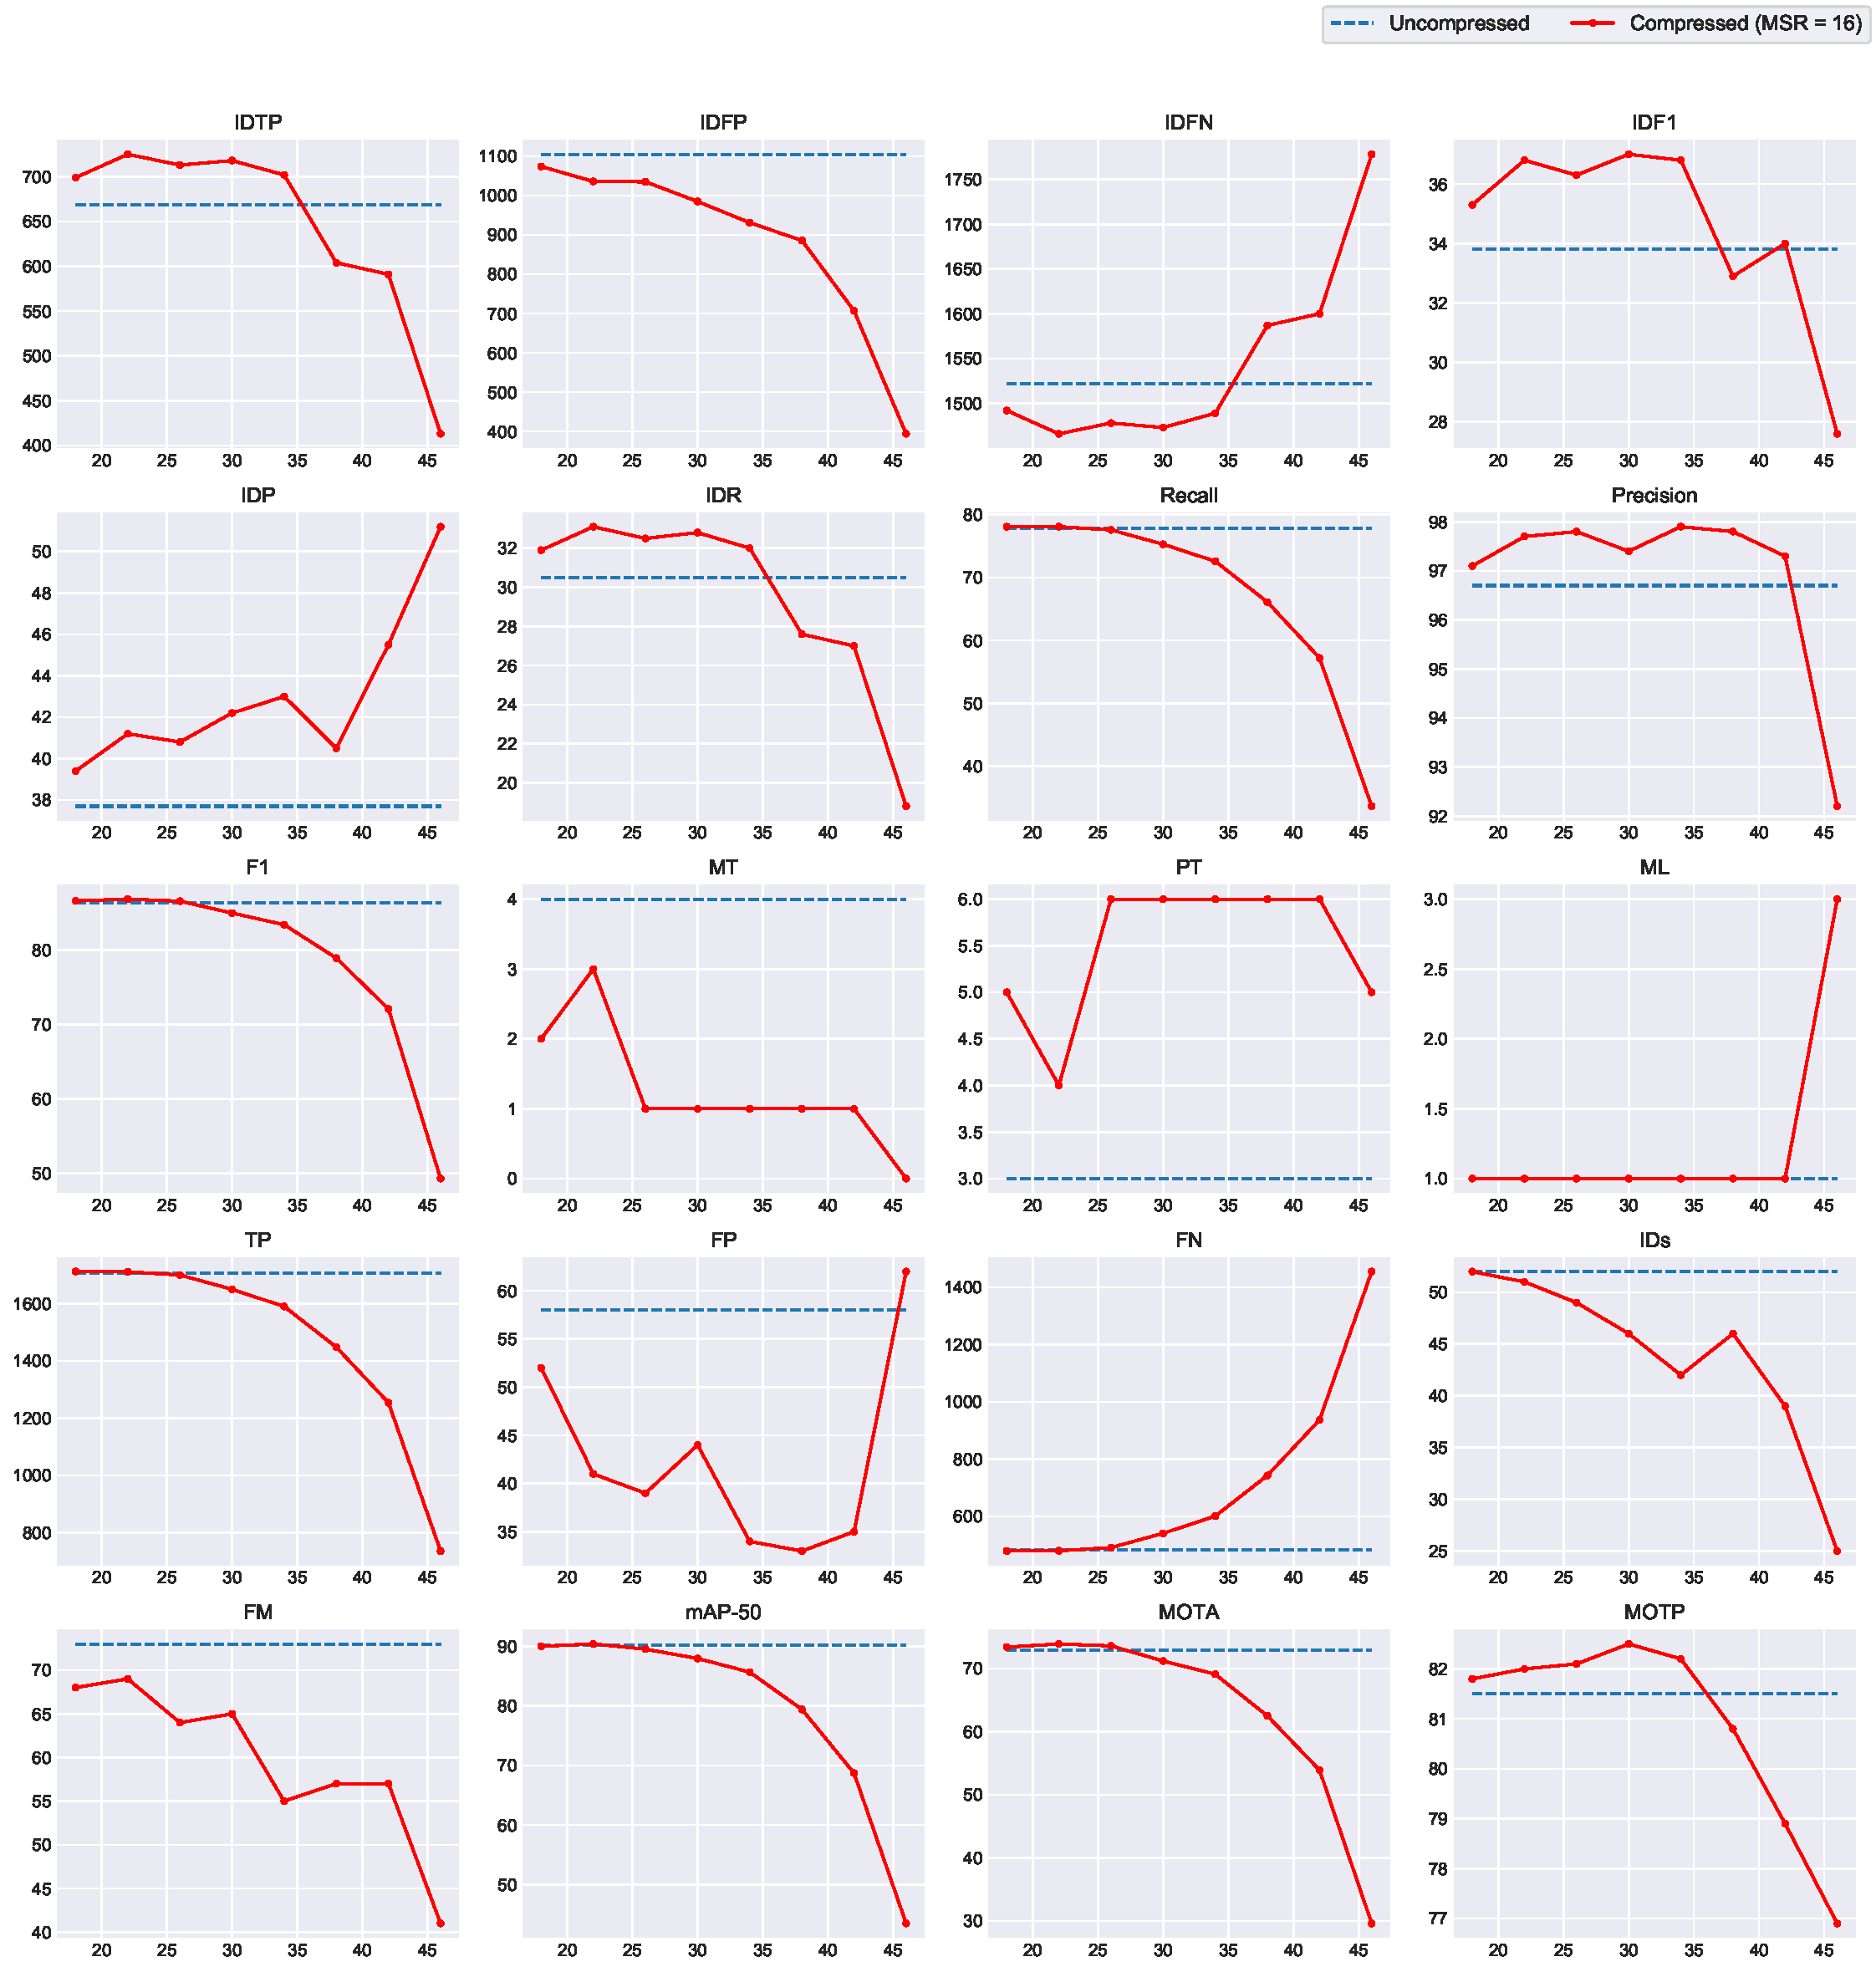
\includegraphics[width=1.0\linewidth]{img/BasketballPass_0_multiplots_qp.pdf}
  \caption[Visualization of the performance results in Class D BasketballPass at different QP for the "person" object class]
  {Visualization of the performance results in Class D BasketballPass at different QP for the "person" object class.
  }
  \label{fig:BasketballPass_0_multiplots_qp}
\end{figure}
\begin{table}[!tb]
    \centering
    \caption[Performance results on BasketballPass]
    {Performance results on BasketballPass.}
    \resizebox{1.0\linewidth}{!}{
\begin{tabular}{llrrrrrrrrrrrrrrrrrrrrr}
\toprule
          QP &          MSR &   IDTP &    IDFP &    IDFN &  IDF1 &   IDP &   IDR &  Recall &  Precision &    F1 &  GT &  MT &  PT &  ML &   TP &  FP &   FN &  IDs &  FM &  mAP-50 &  MOTA &  MOTP \\
\midrule
Uncompressed & Uncompressed & 669.00 & 1105.00 & 1522.00 & 33.80 & 37.70 & 30.50 &   77.90 &      96.70 & 86.29 &   8 &   4 &   3 &   1 & 1707 &  58 &  484 &   52 &  73 &   90.25 & 72.90 & 81.50 \\
          18 &           16 & 699.00 & 1074.00 & 1492.00 & 35.30 & 39.40 & 31.90 &   78.10 &      97.10 & 86.57 &   8 &   2 &   5 &   1 & 1712 &  52 &  479 &   52 &  68 &   90.03 & 73.40 & 81.80 \\
          22 &           16 & 725.00 & 1036.00 & 1466.00 & 36.80 & 41.20 & 33.10 &   78.10 &      97.70 & 86.81 &   8 &   3 &   4 &   1 & 1711 &  41 &  480 &   51 &  69 &   90.42 & 73.90 & 82.00 \\
          26 &           16 & 713.00 & 1035.00 & 1478.00 & 36.30 & 40.80 & 32.50 &   77.60 &      97.80 & 86.54 &   8 &   1 &   6 &   1 & 1700 &  39 &  491 &   49 &  64 &   89.54 & 73.60 & 82.10 \\
          30 &           16 & 718.00 &  985.00 & 1473.00 & 37.00 & 42.20 & 32.80 &   75.30 &      97.40 & 84.94 &   8 &   1 &   6 &   1 & 1650 &  44 &  541 &   46 &  65 &   87.98 & 71.20 & 82.50 \\
          34 &           16 & 702.00 &  931.00 & 1489.00 & 36.80 & 43.00 & 32.00 &   72.60 &      97.90 & 83.37 &   8 &   1 &   6 &   1 & 1590 &  34 &  601 &   42 &  55 &   85.69 & 69.10 & 82.20 \\
          38 &           16 & 604.00 &  886.00 & 1587.00 & 32.90 & 40.50 & 27.60 &   66.10 &      97.80 & 78.88 &   8 &   1 &   6 &   1 & 1448 &  33 &  743 &   46 &  57 &   79.42 & 62.50 & 80.80 \\
          42 &           16 & 591.00 &  707.00 & 1600.00 & 34.00 & 45.50 & 27.00 &   57.20 &      97.30 & 72.05 &   8 &   1 &   6 &   1 & 1254 &  35 &  937 &   39 &  57 &   68.72 & 53.90 & 78.90 \\
          46 &           16 & 413.00 &  394.00 & 1778.00 & 27.60 & 51.20 & 18.80 &   33.60 &      92.20 & 49.25 &   8 &   0 &   5 &   3 &  736 &  62 & 1455 &   25 &  41 &   43.45 & 29.60 & 76.90 \\
\bottomrule
\end{tabular}
    }
    \label{tab:BasketballPass_0}
\end{table}
The result is consistent with the averaged result shown in Chapter \ref{sec:results/section_a} such that the performance decreases as QP increases on most of the metrics except IDP and MOTP. To examine the result more thoroughly, we inspected the video sequence in frame by frame at different QP. 


\subsection{Case II: Class D BlowingBubbles}